\documentclass[9pt]{beamer}
\mode<presentation>
\usepackage[T1]{fontenc}
\usepackage{color}
\usepackage{graphicx}
\usepackage{natbib}
\usepackage{tikz}
\usetikzlibrary{shapes.geometric}
\usepackage{xmpmulti}
\usepackage{animate}
\usepackage{tcolorbox}
\usepackage{amsmath}
\usepackage{gensymb}
\usepackage{csquotes}
\usepackage{bibentry}
\nobibliography*

%\usetheme{Singapore}
%\usecolortheme{seahorse}

\usefonttheme{professionalfonts}

\title[Word \& Doc Embeddings]{A Rapid Computer-assisted Systematic Map of Regional Climate Impacts - Results [1]}
%\author{Max Callaghan, Gerritt }
\institute[MCC]{
	
\includegraphics[height=1cm,width=2cm]{images/MCC_Logo_RZ_rgb.jpg} \hspace{5em} 
\includegraphics[height=1cm]{images/climate_analytics.png}
}

\newif\ifframeinlbf
\frameinlbftrue
\makeatletter
\newcommand\listofframes{\@starttoc{lbf}}
\makeatother

\addtobeamertemplate{frametitle}{}{%
	\ifframeinlbf
	\addcontentsline{lbf}{section}{\protect\makebox[2em][l]{%
			\protect\usebeamercolor[fg]{structure}\insertframenumber\hfill}%
		\insertframetitle\par}%
	\else\fi
}

\newtheorem*{remark}{}

\bibliographystyle{apalike}

\begin{document}
	
\begin{frame}
	\titlepage
\end{frame}

\begin{frame}{Outline}

\tableofcontents

\end{frame}

\section{Recap - Goal}
\begin{frame}{Goal}
There are hundreds of thousands of documents potentially relevant to observed climate impacts. We want to be able to do two things:

\begin{itemize}
	\item Separate those documents which \textit{are} relevant from those that are not
	\item Predict in what way relevant documents are relevant:
	\begin{itemize}
		\item What impacts do they document?
		\item What type of evidence do they provide?
		\item In which locations is there evidence
	\end{itemize}
\end{itemize}

Once we can do that, we can draw a rough map of the available evidence, and/or aid the production of an \textit{assessment} of the available evidence 

\end{frame}

\begin{frame}{Context}

Systematic assessments of the evidence on Climate Change like those conducted by the IPCC are vital.

\begin{columns}
	\begin{column}{0.618\linewidth}
		\begin{figure}
			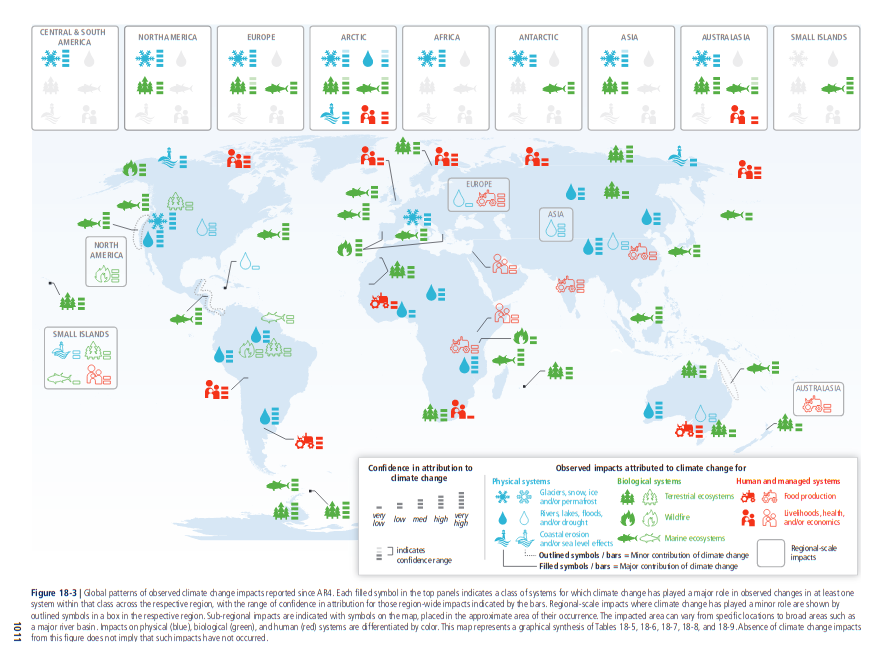
\includegraphics[width=\linewidth]{../map_18.png}<1->
		\end{figure}
	\end{column}
	\begin{column}{0.312\linewidth}
		
		\begin{figure}
			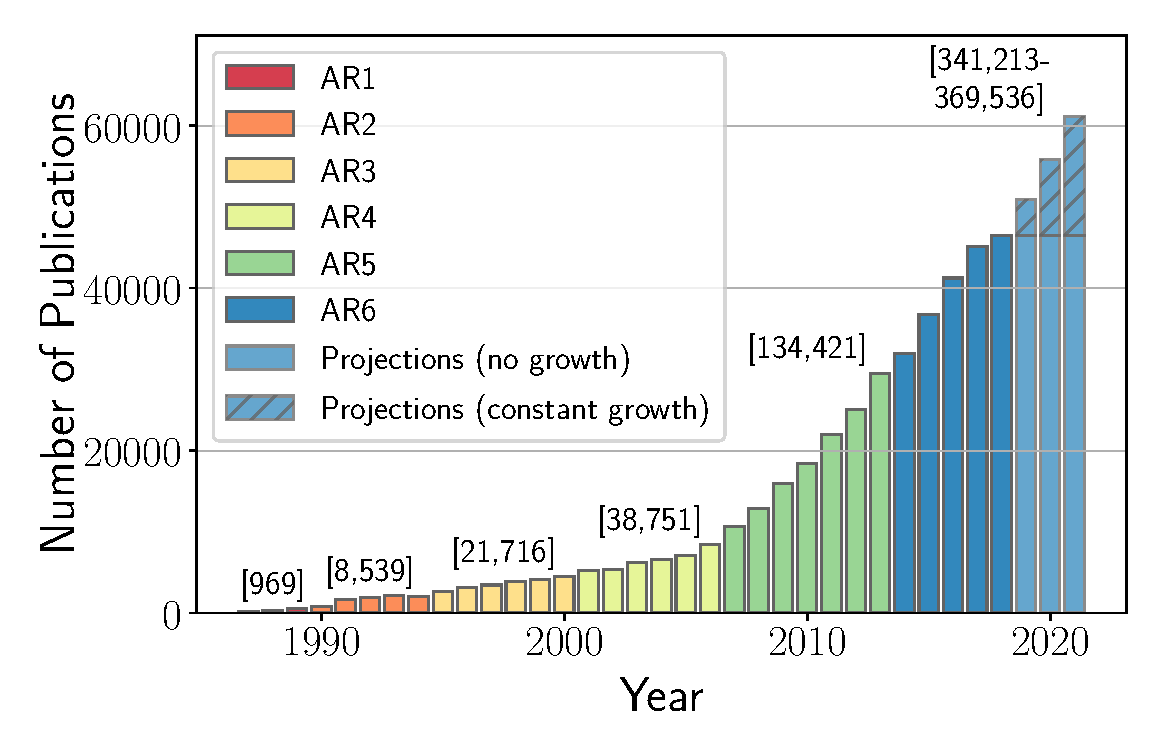
\includegraphics[width=\linewidth]{images/pubs_time_wgb_lp.pdf}<2->
		\end{figure}
		
		\begin{itemize}
			\small
			\item<2->These are challenged by big literature 
			\item<3->They do not account for uncertainty about what literature is available
		\end{itemize}
	\end{column}
\end{columns}

\end{frame}



\begin{frame}{Distribution of labour between humans and machines}

A human expert or a team of human experts is best placed to answer those questions for any single document, but they can't look at all potentially relevant documents

\bigskip

We can use labels generated by humans to try to teach a computer what a relevant document looks like, and how to decide in what way it is relevant. 

\bigskip

If this works well, we can predict, with some uncertainty, how much evidence there is, and where and on what topic it is.

\end{frame}

\section{Data collection}
\begin{frame}
\tableofcontents[currentsection]
\end{frame}

\begin{frame}{Over the last month and a half we screened 1500 documents}

\begin{figure}
	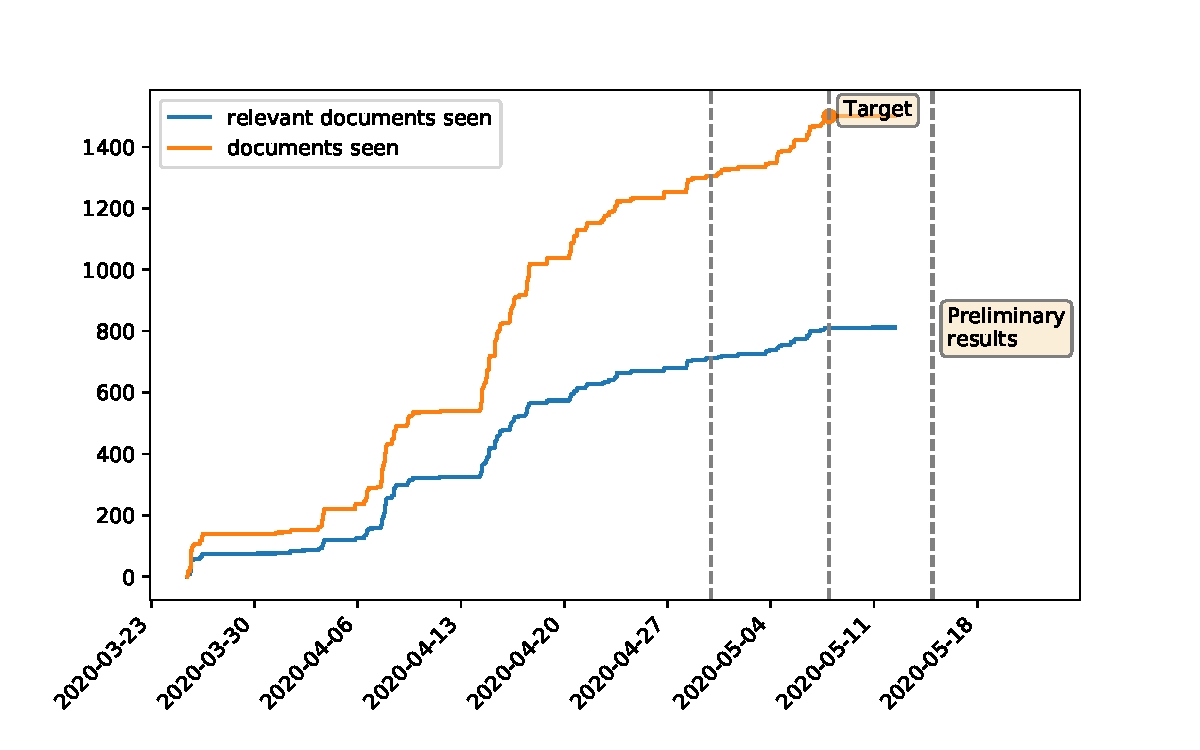
\includegraphics[width=\linewidth]{../plots/progress/plan.pdf}
\end{figure}

\end{frame}

\begin{frame}{This already constitutes a useful information gathering exercise}

\begin{figure}
	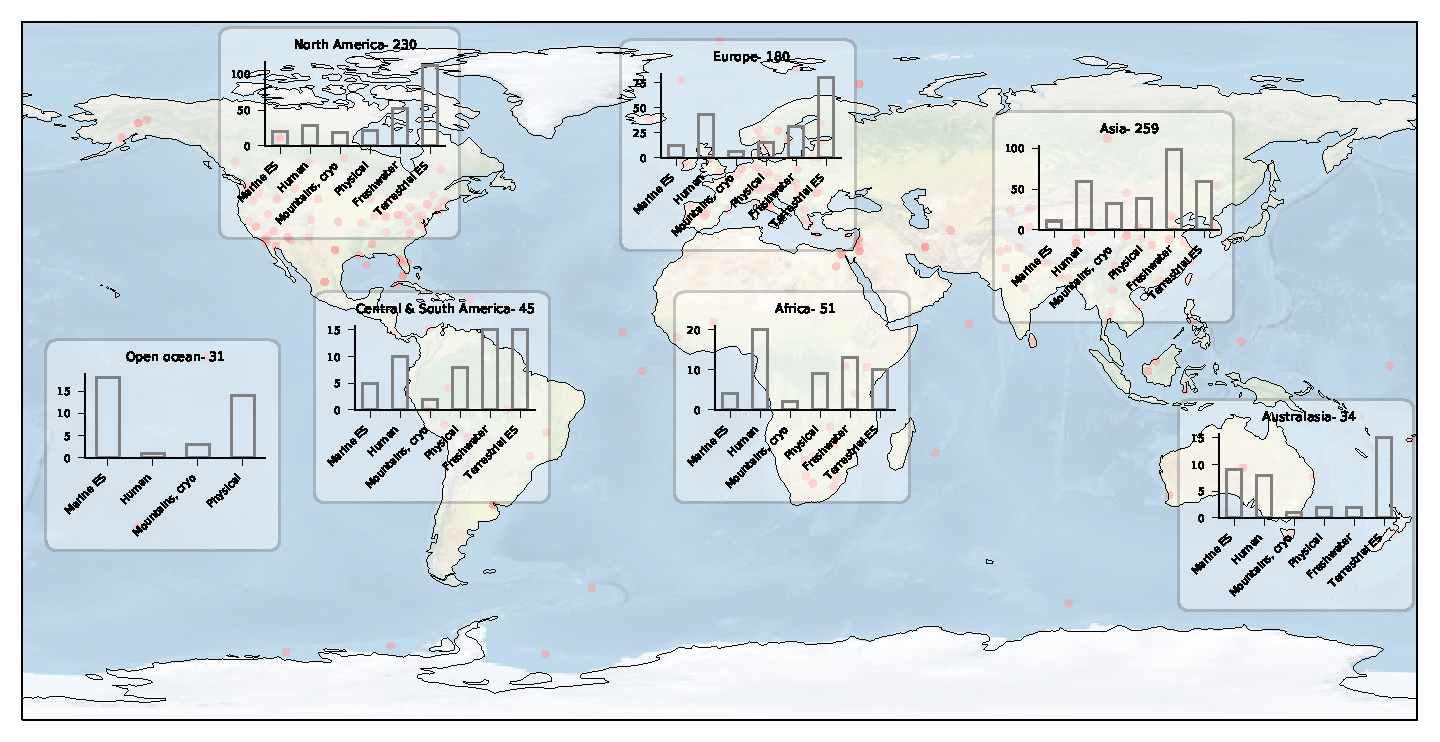
\includegraphics[width=\linewidth]{../plots/map_coded.pdf}
\end{figure}

\end{frame}

\section{Outcome 1 - prediction performance}
\begin{frame}
\tableofcontents[currentsection]
\end{frame}

%\begin{frame}{Other Data}
%
%In addition to what we collected together we also have other coded documents:
%
%\bigskip
%
%\begin{columns}[t]
%	\begin{column}{0.5\linewidth}
%		AR5 Data 256 documents we can use to supplement our training set
%	\end{column}
%	\begin{column}{0.5\linewidth}
%		700 Documents I coded earlier this year.
%		
%		500 are a random sample we can use for validation
%	\end{column}
%\end{columns}
%\end{frame}

\begin{frame}{We predict the relevance of a document most of the time}
\begin{figure}
	\begin{columns}
		\begin{column}{0.3812\linewidth}
			\begin{figure}
					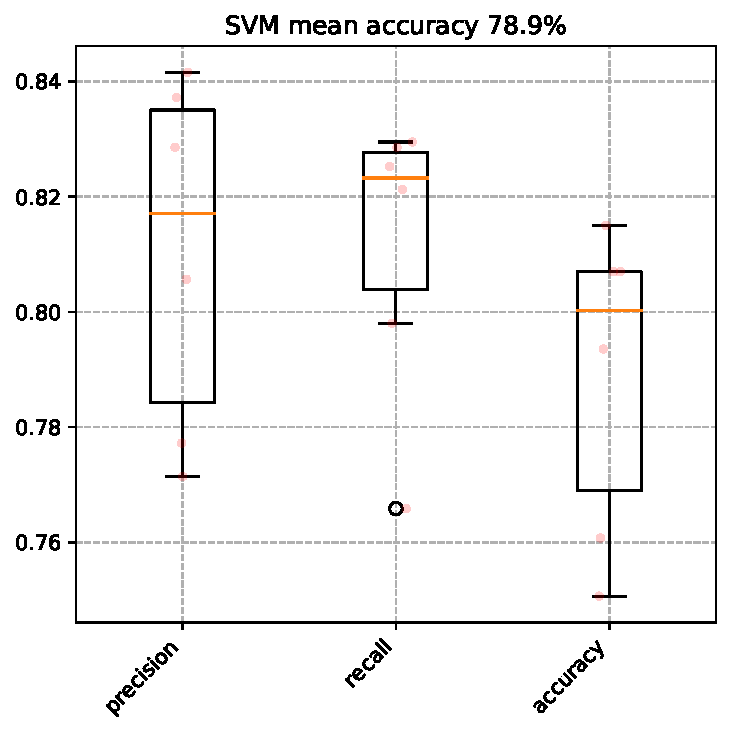
\includegraphics[width=\linewidth]{../plots/prediction_models/relevance_prediction_2020-05-12.pdf}
			\end{figure}
			\begin{figure}
				\only<1>{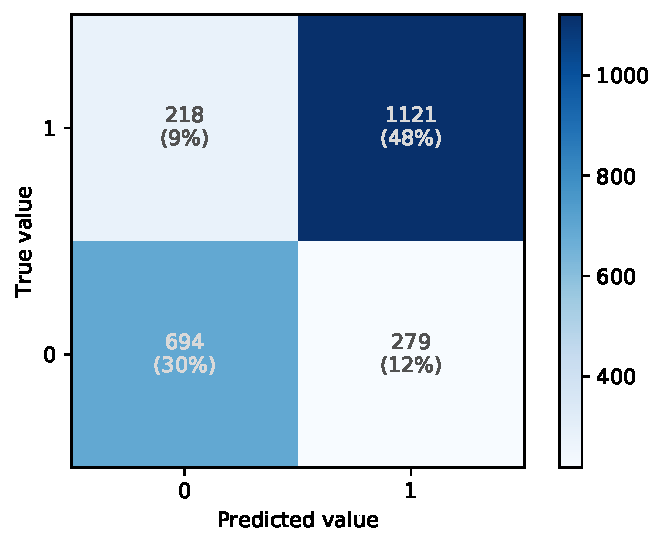
\includegraphics[width=\linewidth]{../plots/prediction_models/relevance_confusion.pdf}}
				\only<2>{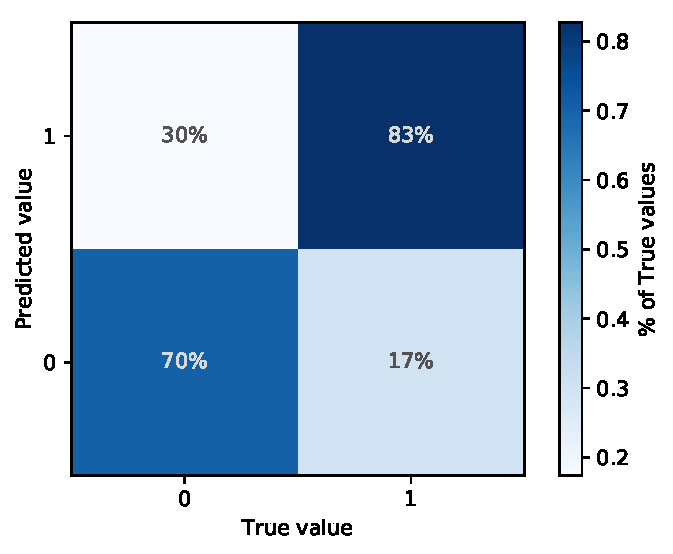
\includegraphics[width=\linewidth]{../plots/prediction_models/relevance_confusion_true.pdf}}
				\only<3>{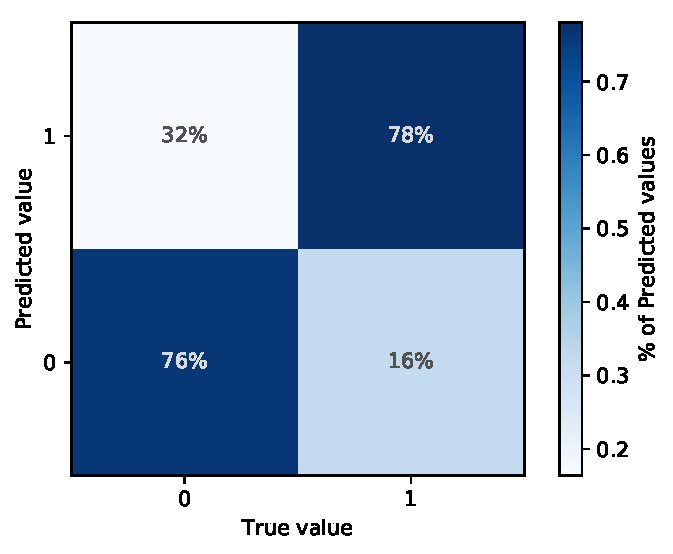
\includegraphics[width=\linewidth]{../plots/prediction_models/relevance_confusion_pred.pdf}}
			\end{figure}
		\end{column}
		\begin{column}{0.5\linewidth}
			This has been steadily increasing by using the model itself as a "second pair of eyes" to check for errors, and I expect it to increase further (partly due to different criteria for inclusion at different stages of the project)
		\end{column}
	\end{columns}

\end{figure}
\end{frame}


\begin{frame}{We can clearly identify what impact category a document is related to}

\begin{figure}
	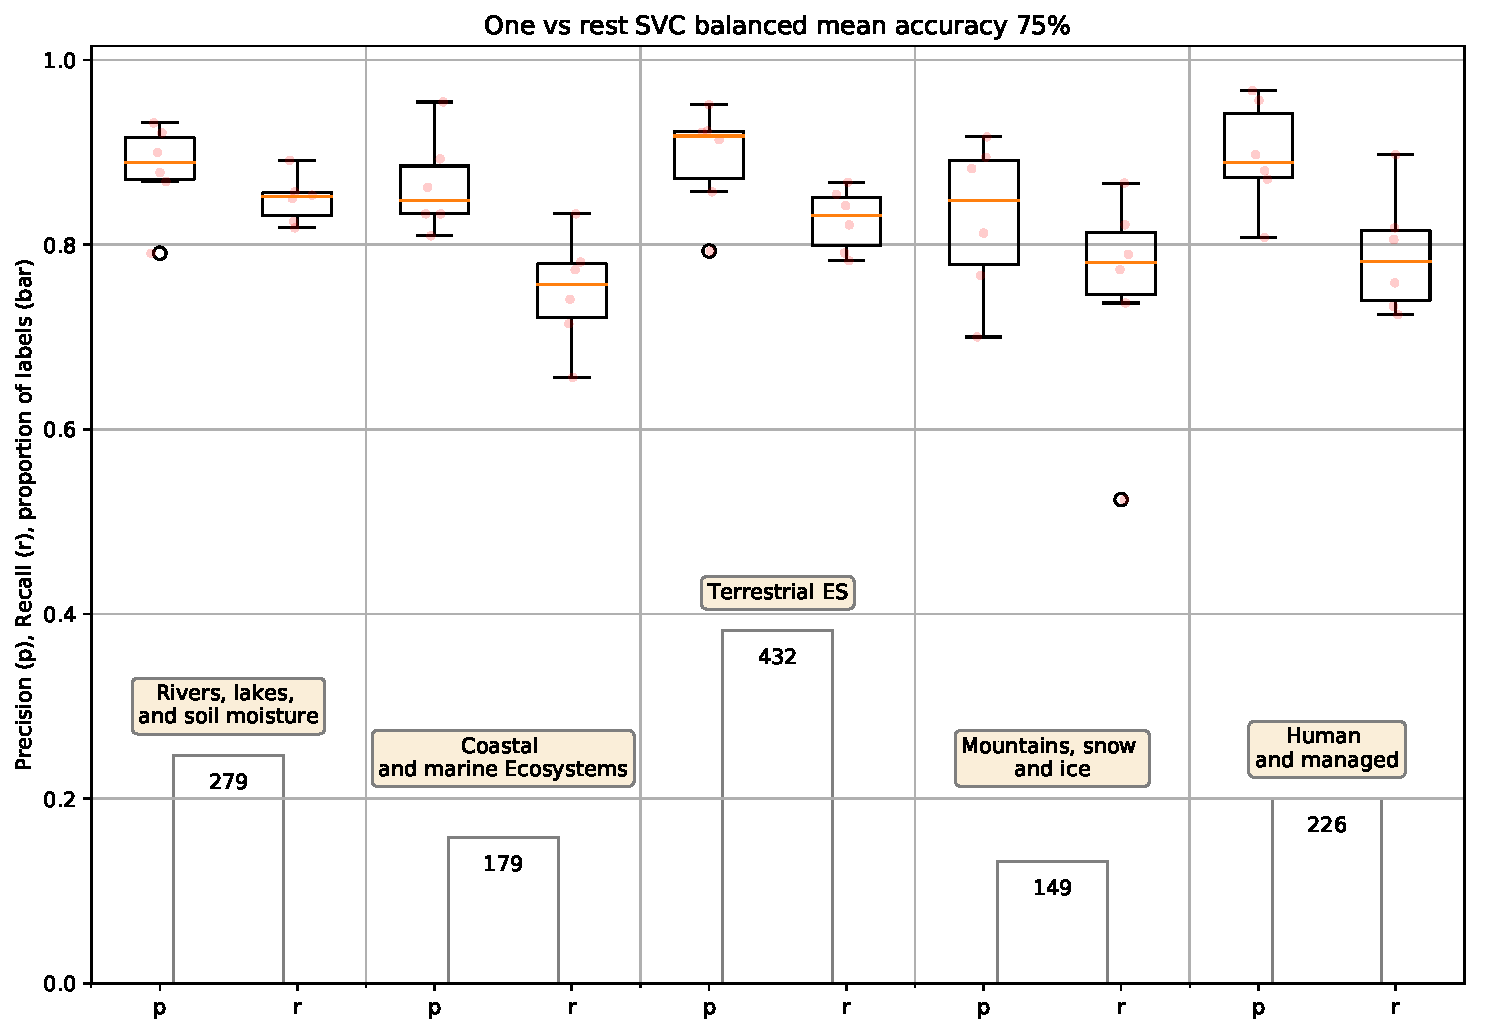
\includegraphics[width=0.9\linewidth]{../plots/progress/cats_prediction.pdf}
	\caption{Precision (how many documents predicted to be in a category actually had that label) and Recall (how many documents with a label were predicted to be in that category) for each broad impact category}
\end{figure}

\end{frame}

\begin{frame}{We can clearly identify what impact category a document is related to}

\begin{figure}
	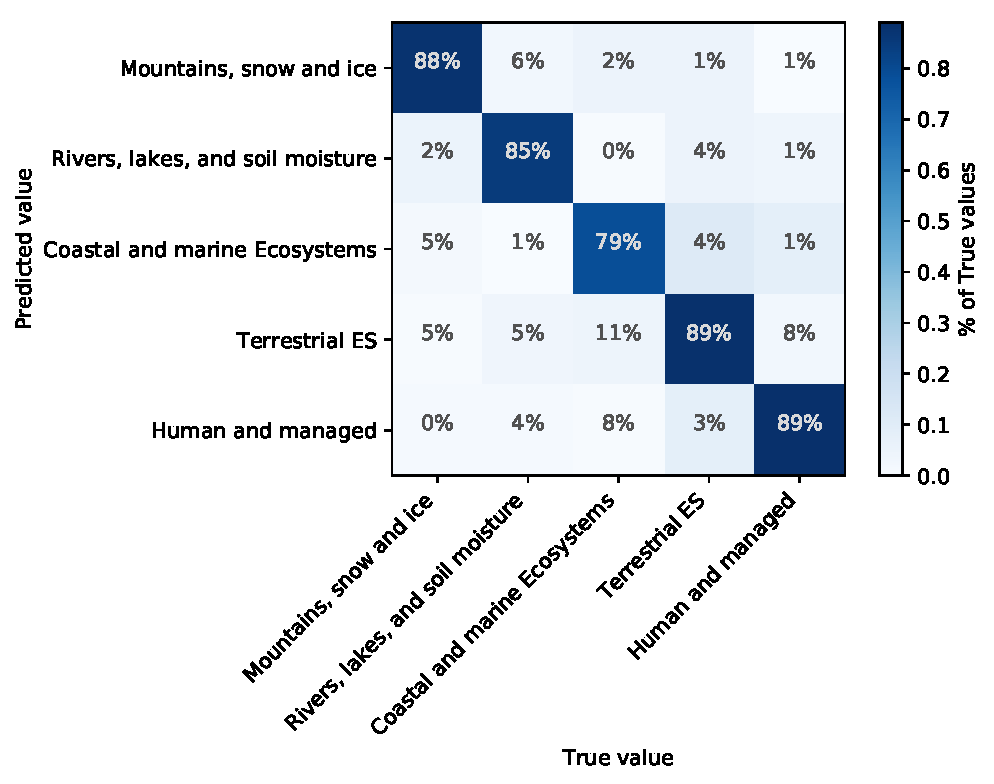
\includegraphics[width=0.9\linewidth]{../plots/prediction_models/category_confusion.pdf}
\end{figure}

\end{frame}



\begin{frame}{Accuracy and uncertainty increased with the number of labels available}

\begin{figure}
	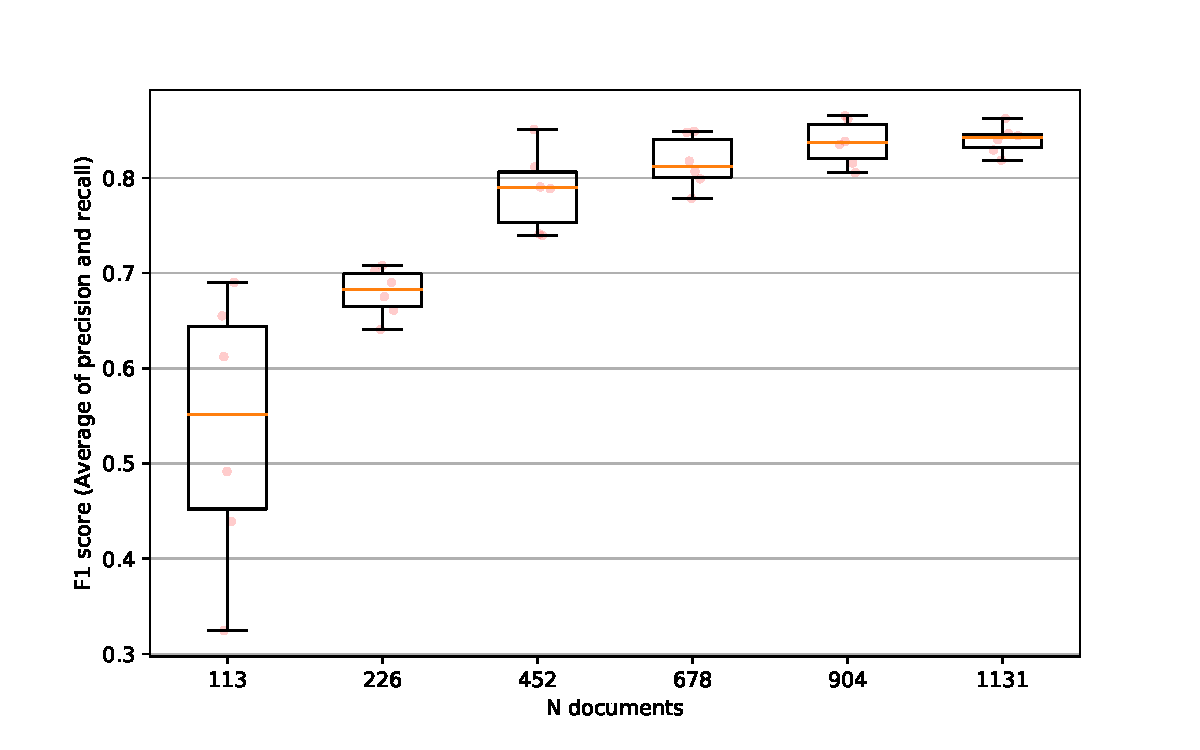
\includegraphics[width=0.8\linewidth]{../plots/progress/cats_prediction_n.pdf}

\end{figure}

\end{frame}

\begin{frame}{We are also broadly correct on subcategories - impressive given the amount of data and the complexity of the coding scheme}
	\begin{figure}
		
		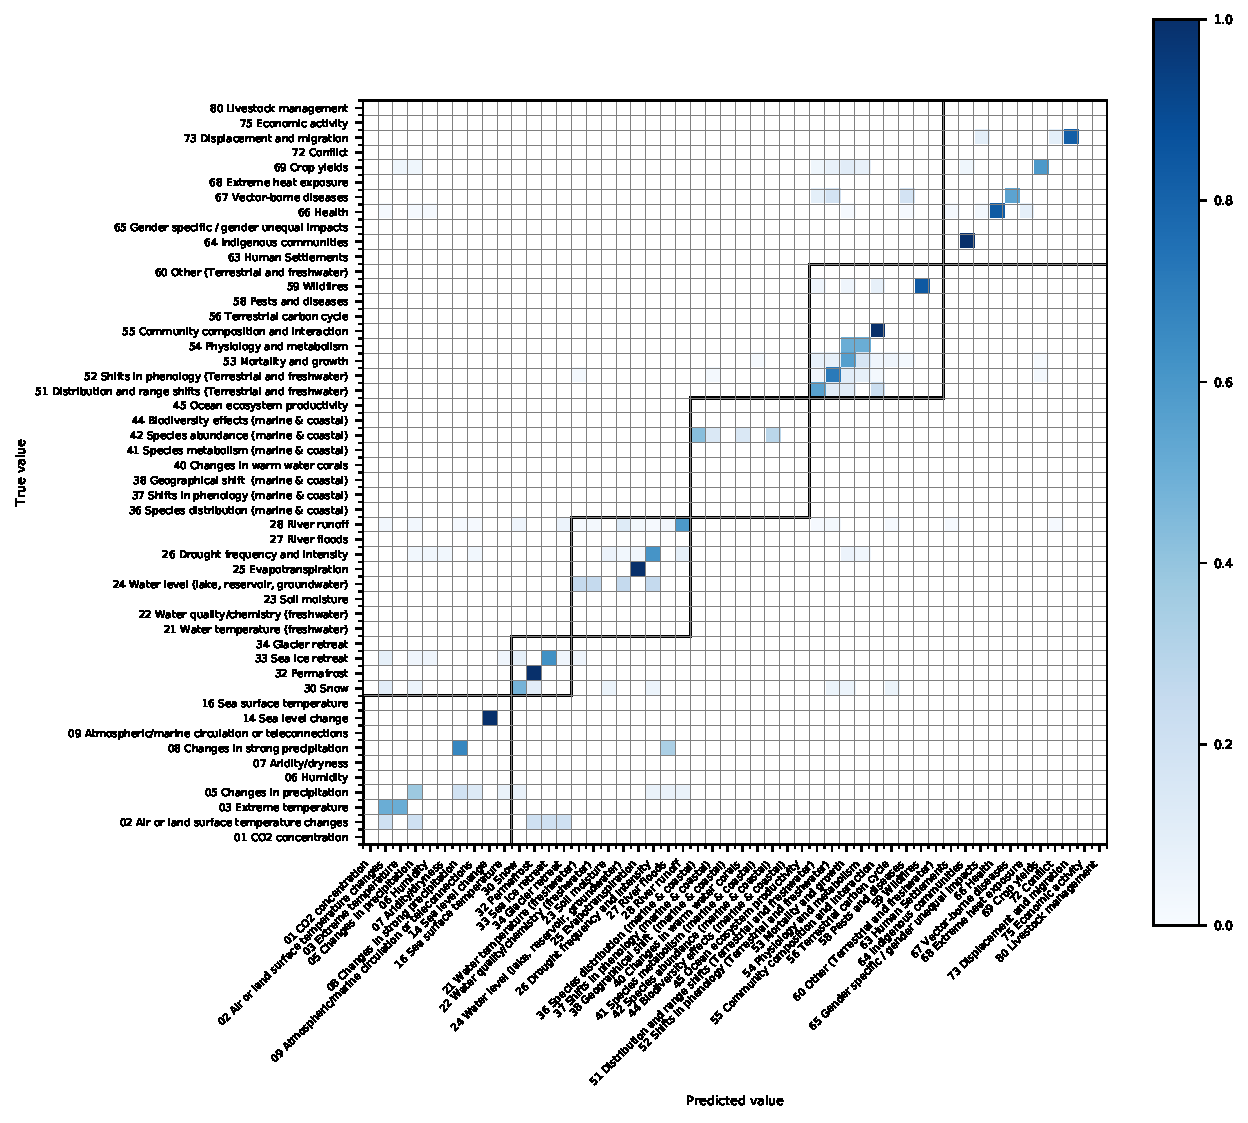
\includegraphics[width=0.8\linewidth]{../plots/prediction_models/confusion_all_classes_pred.pdf}
	\end{figure}
\end{frame}

\begin{frame}{Getting attribution correct is harder, but we have fewer labels}
	\begin{figure}
	
	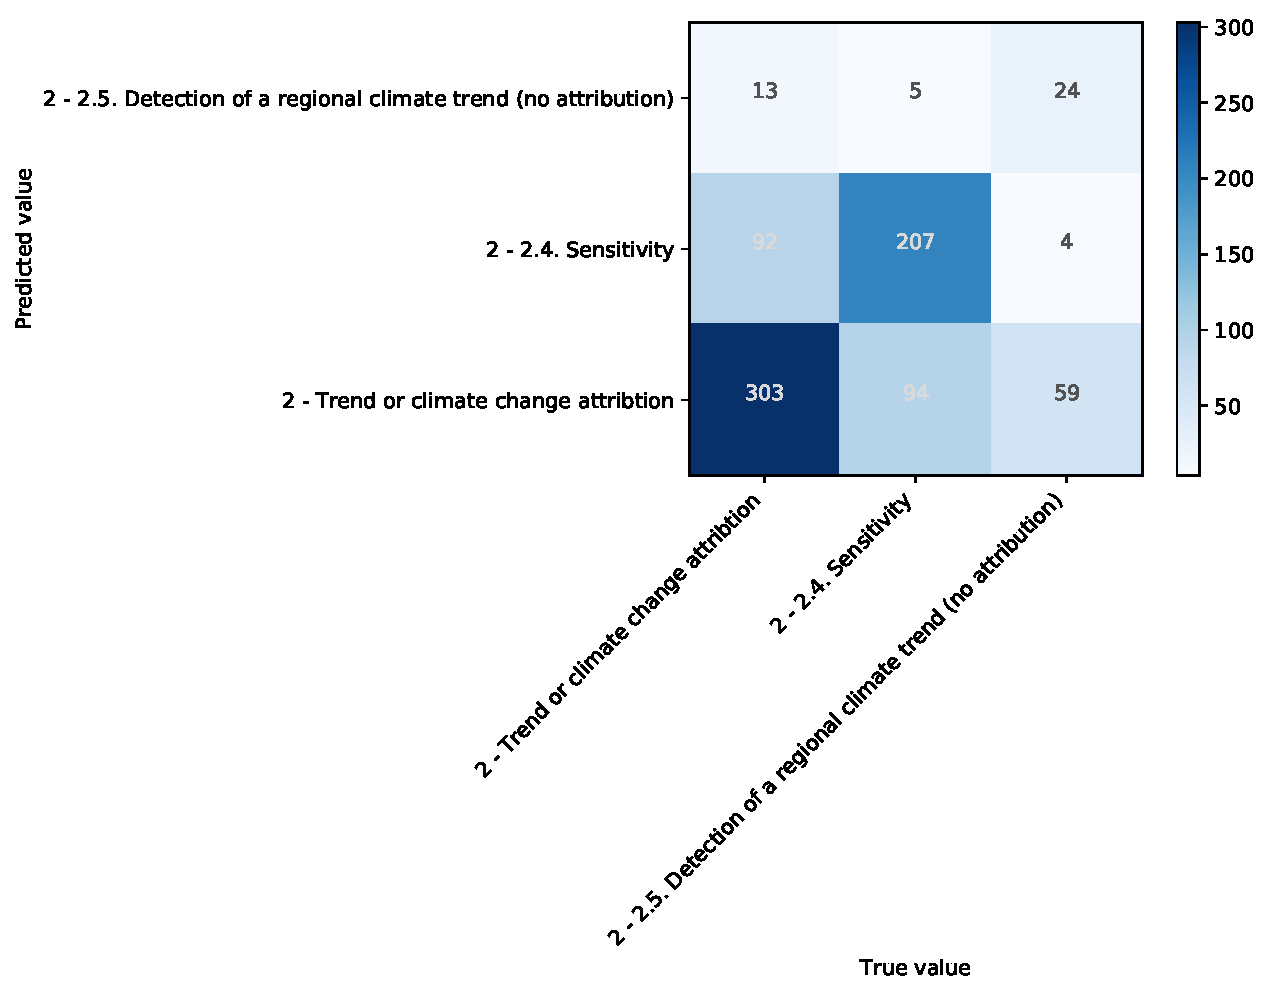
\includegraphics[width=0.8\linewidth]{../plots/prediction_models/confusion_attribution.pdf}
	\end{figure}
\end{frame}


\section{Outcome 2 - Evidence Map}
\begin{frame}
\tableofcontents[currentsection]
\end{frame}

\begin{frame}{We predict tens of thousands of additional documents relevant according to the criteria we defined}
	\begin{figure}
		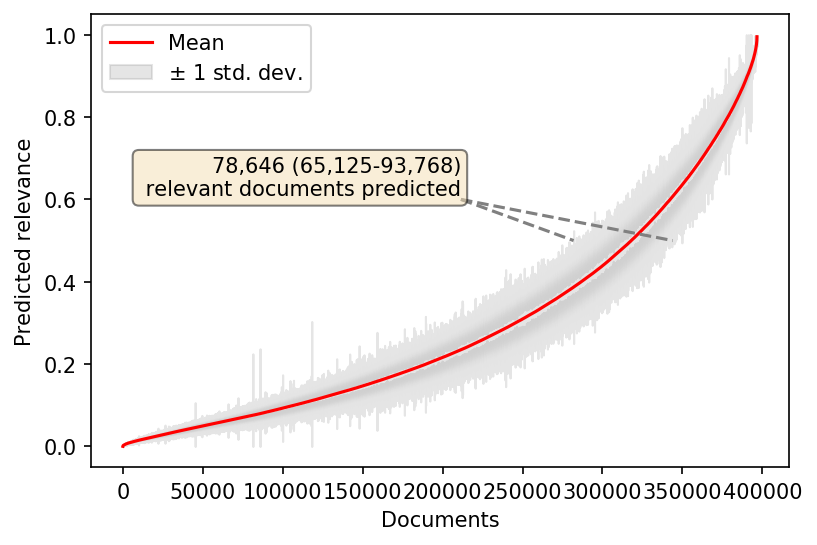
\includegraphics[width=\linewidth]{../plots/prediction_models/predictions_unseen.png}
	\end{figure}
\end{frame}

\begin{frame}
\only<1>{
	\begin{figure}
		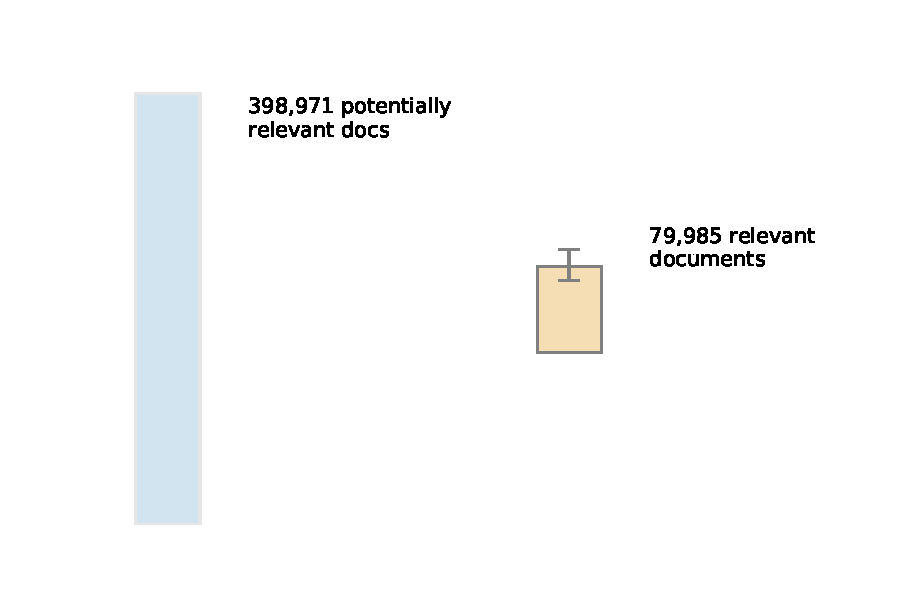
\includegraphics[width=0.7\linewidth]{../plots/process_diagram/relevant.pdf}
	\end{figure}
}
\only<2>{
	\begin{figure}
		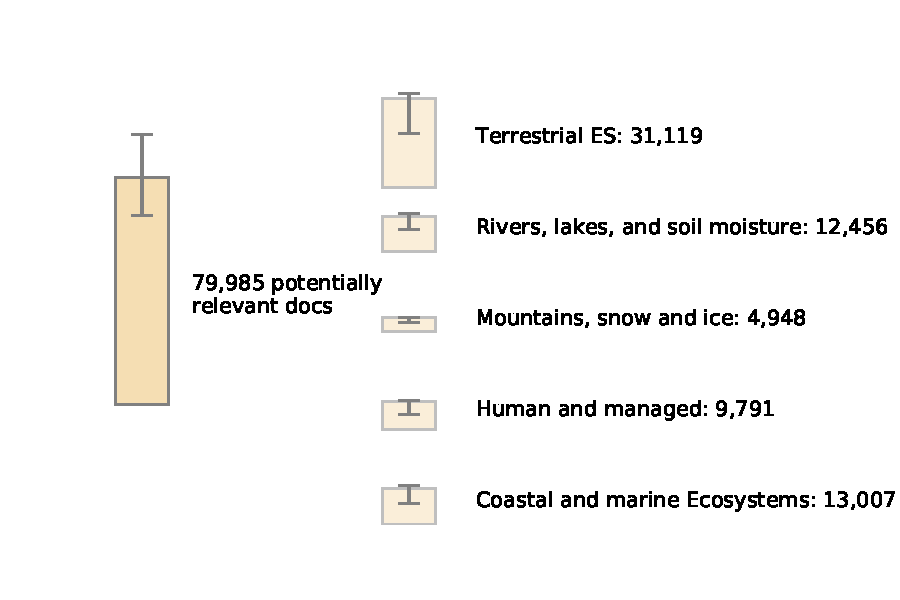
\includegraphics[width=0.7\linewidth]{../plots/process_diagram/relevant_cats.pdf}
	\end{figure}
}
\only<3>{
	\begin{figure}
		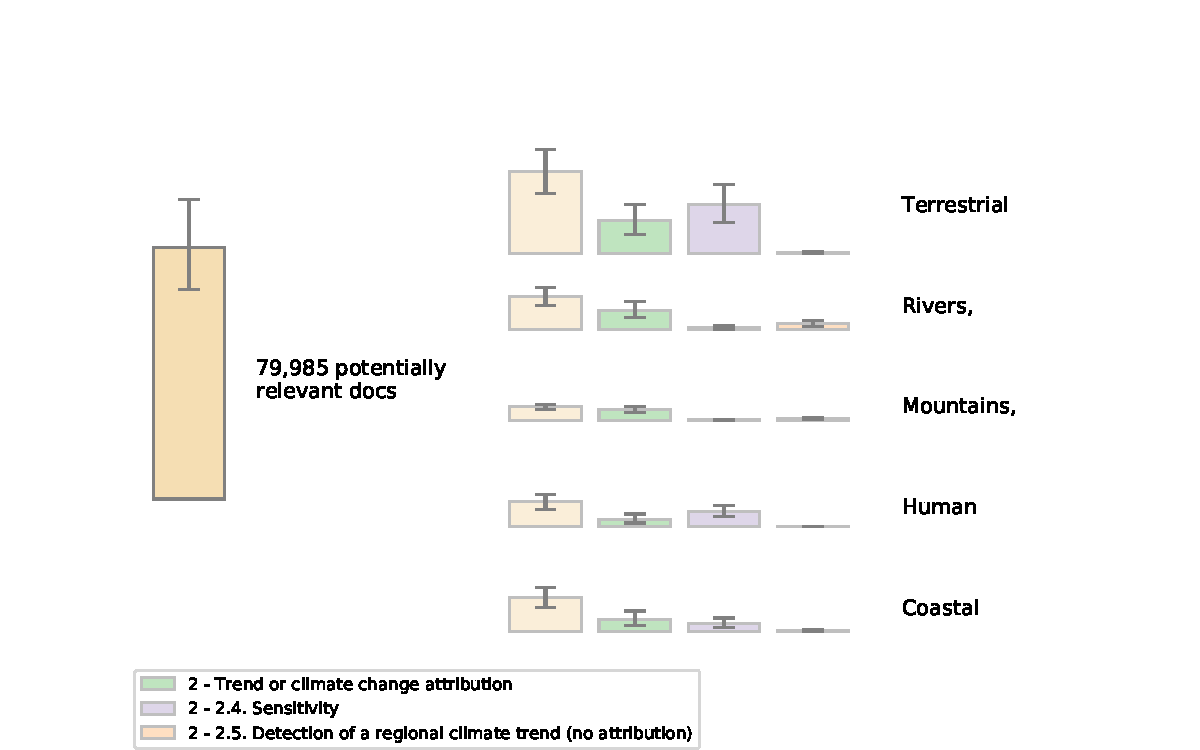
\includegraphics[width=0.7\linewidth]{../plots/process_diagram/relevant_cats_attrib.pdf}
	\end{figure}
}
\end{frame}

\begin{frame}{The studies predicted to be relevant cover a much broader array of places, but geographic imbalances persist}
\only<1>{
	\begin{figure}
	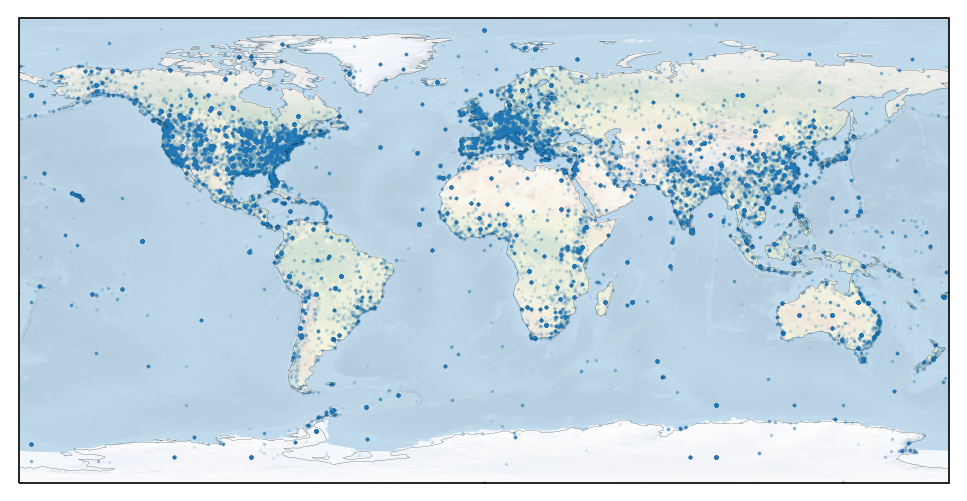
\includegraphics[width=\linewidth]{../plots/maps/all_predicted_places.png}
\end{figure}
}
\only<2>{
	\begin{figure}
		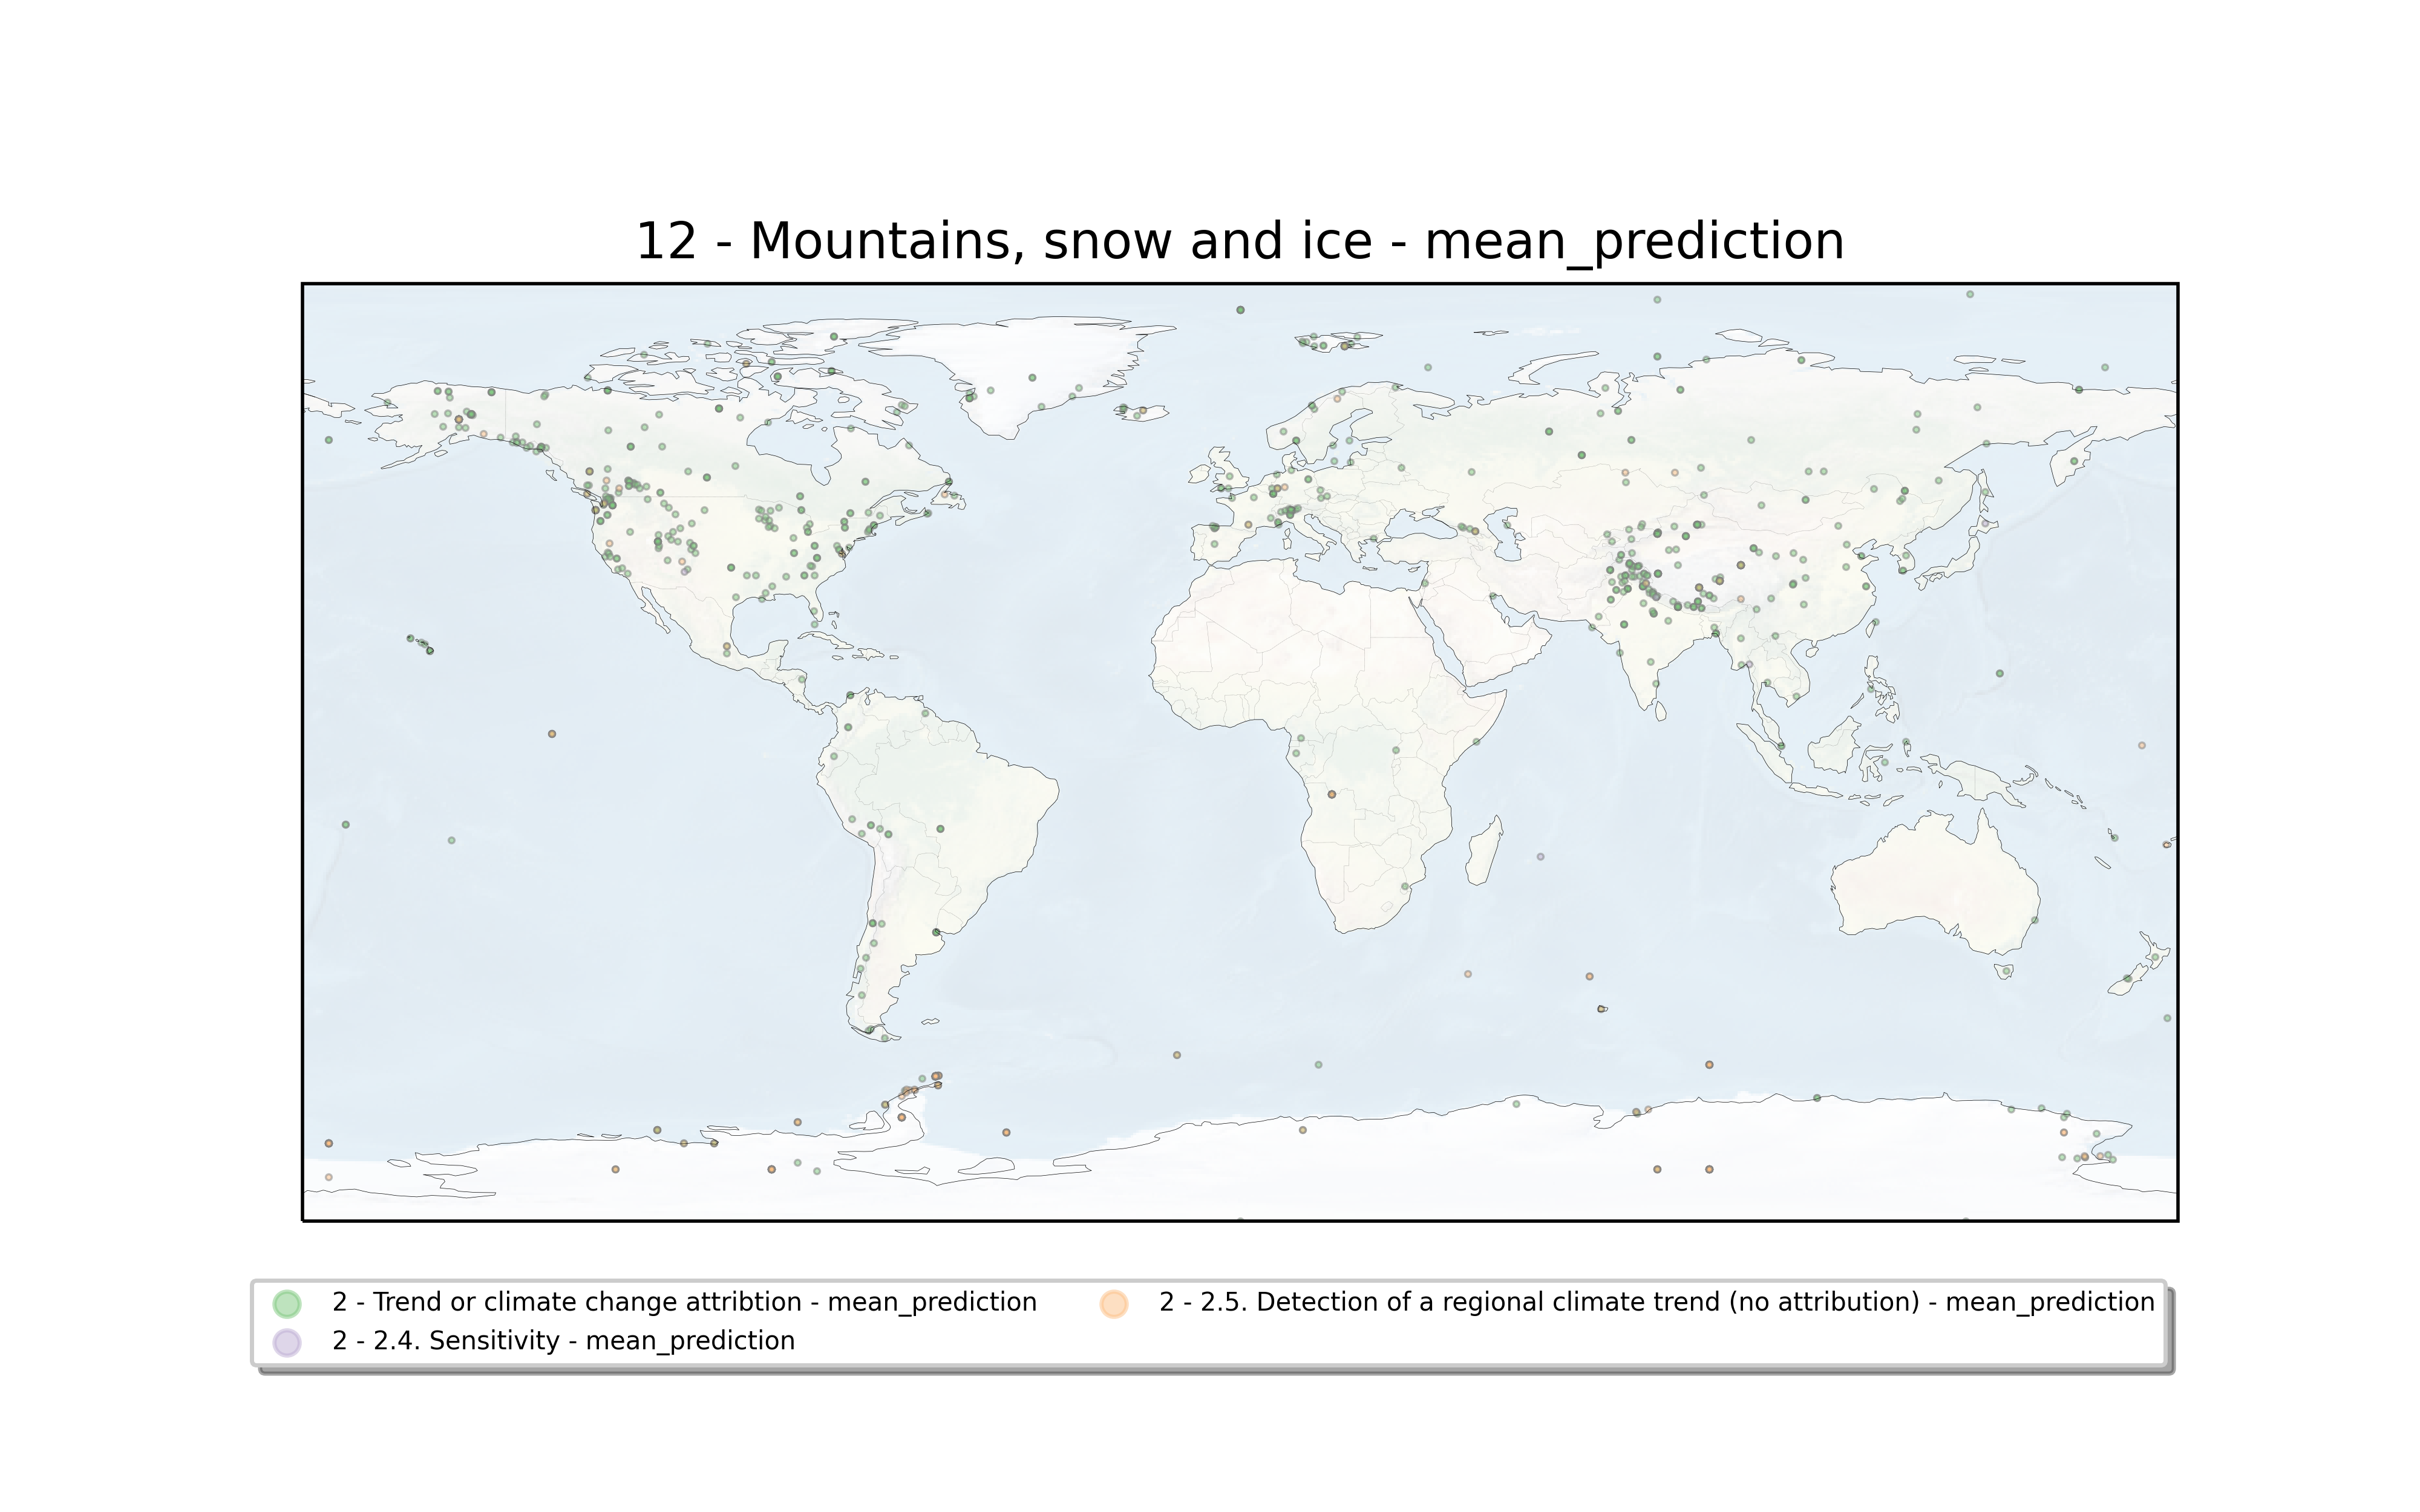
\includegraphics[width=\linewidth]{../plots/maps/predicted_places_Mountains,_snow_and_ice_attribution.png}
	\end{figure}
}
\only<3>{
	\begin{figure}
		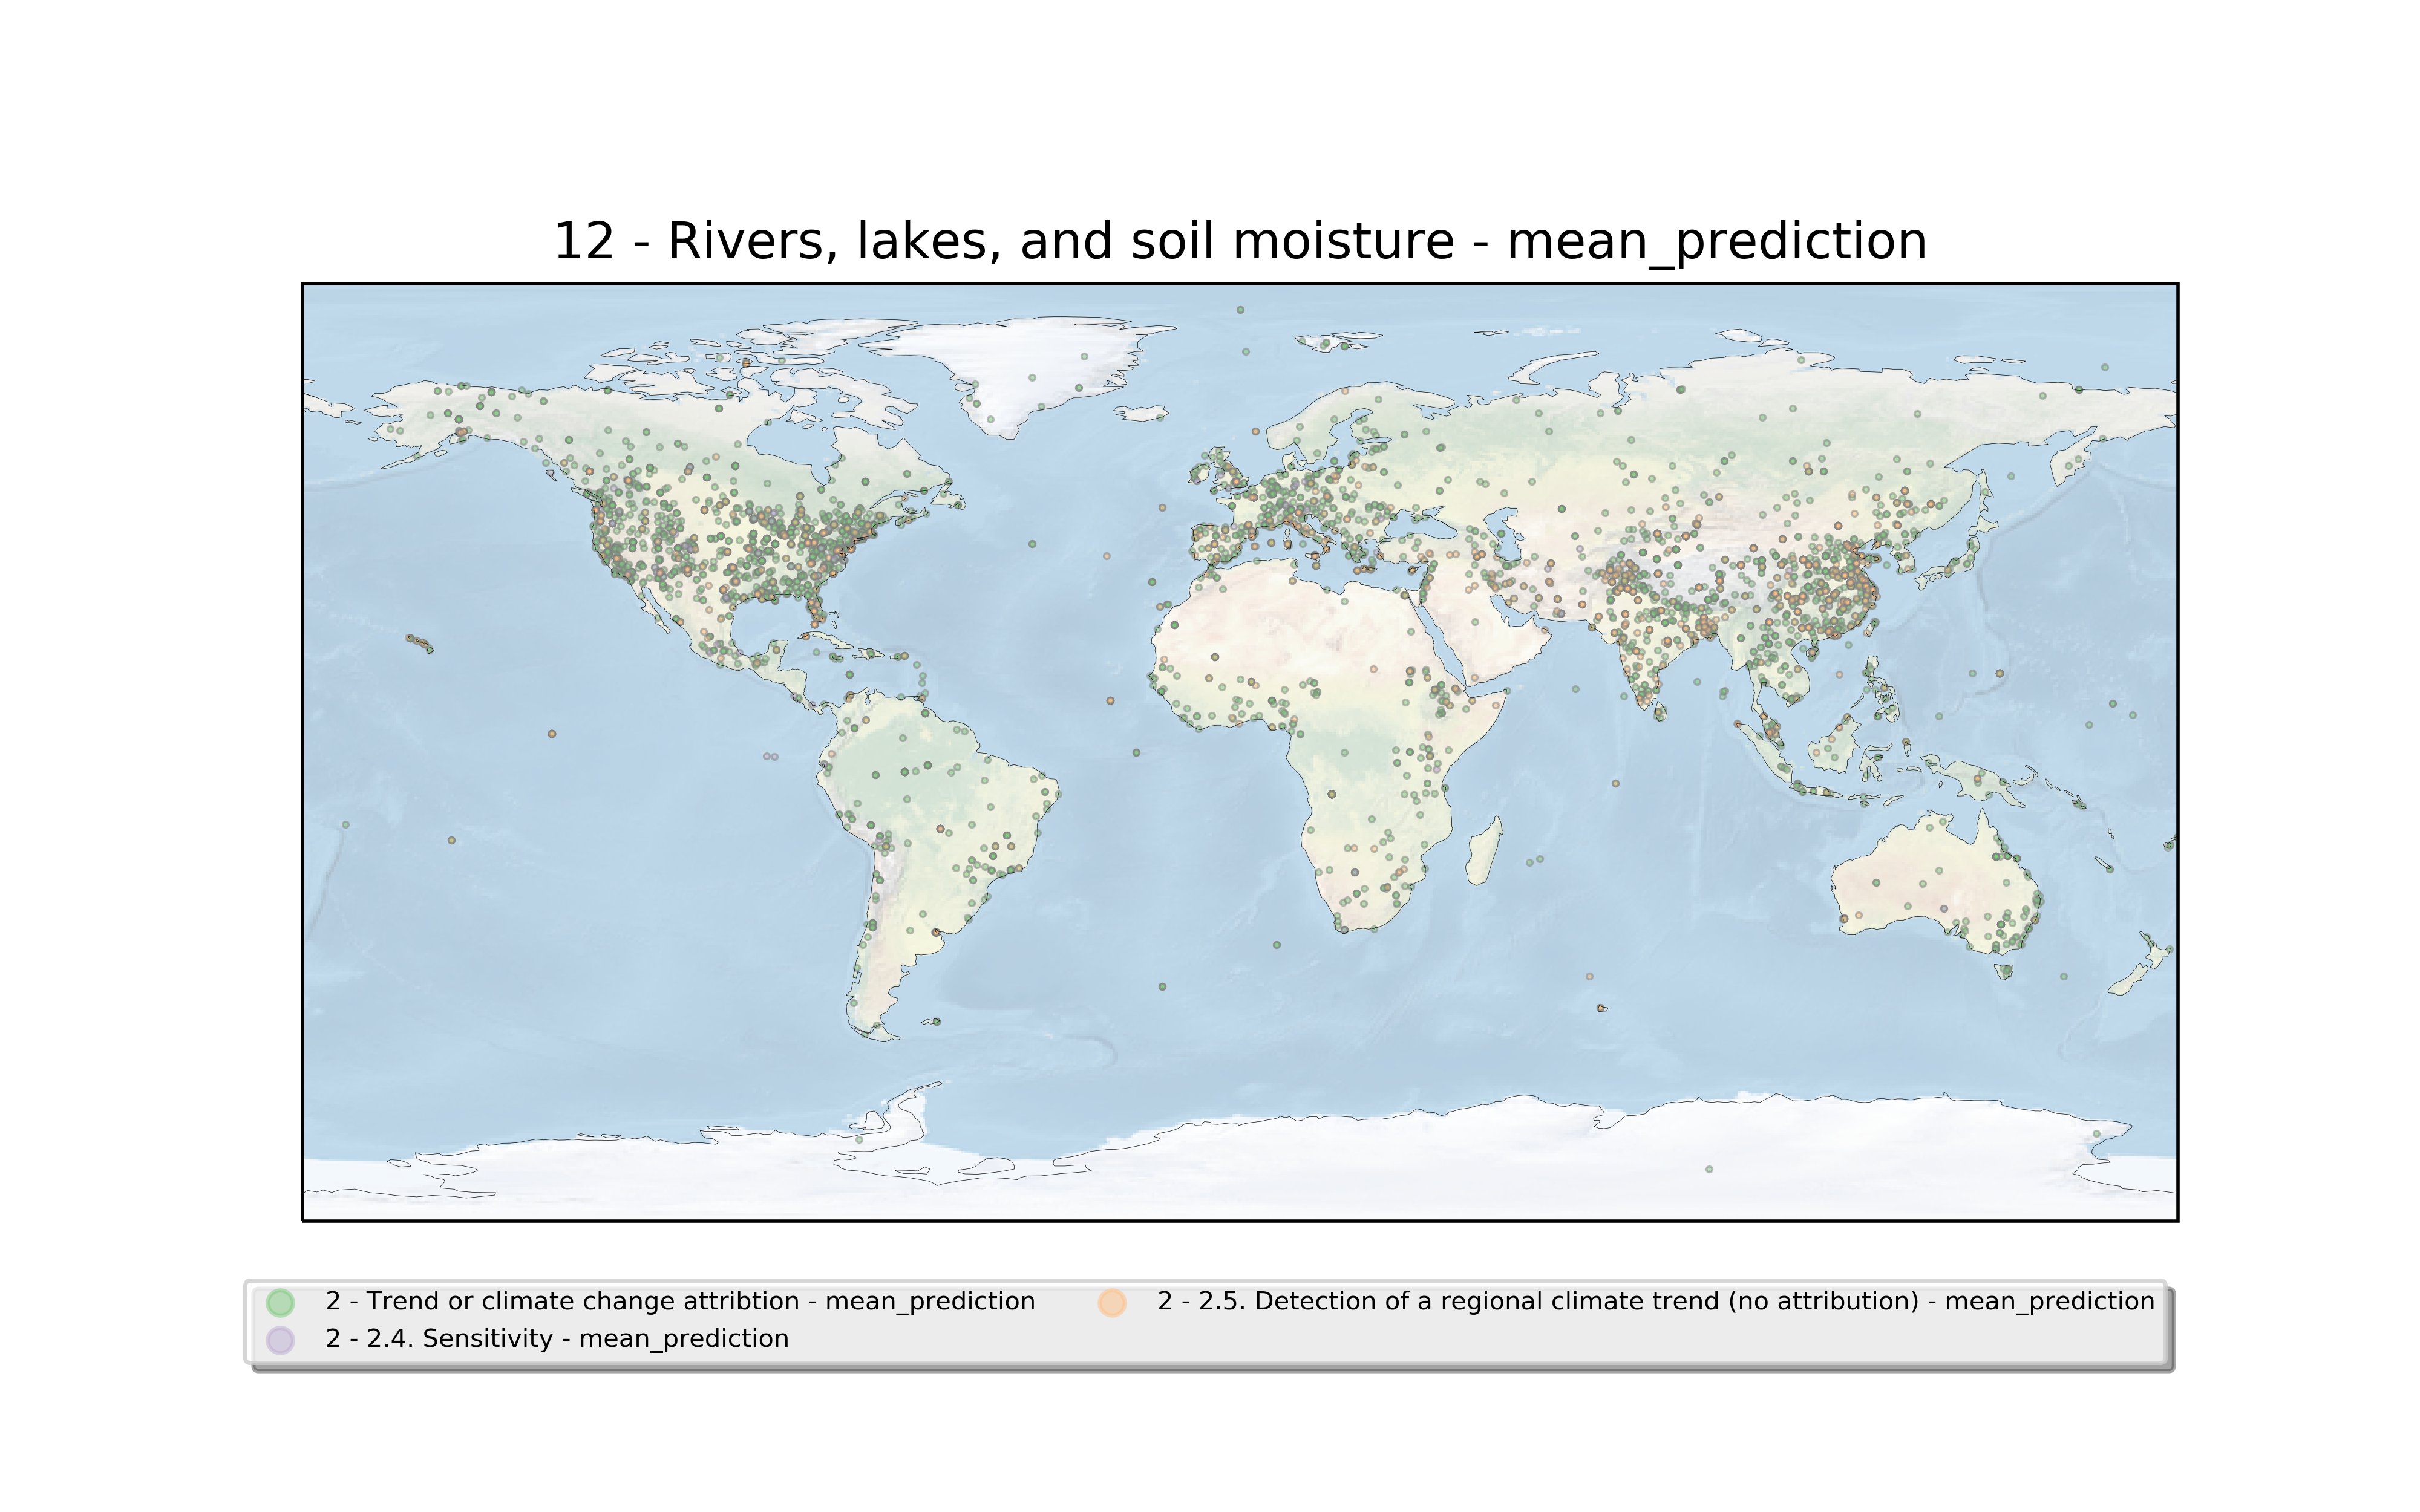
\includegraphics[width=\linewidth]{../plots/maps/predicted_places_Rivers,_lakes,_and_soil_moisture_attribution.png}
	\end{figure}
}
\only<4>{
	\begin{figure}
		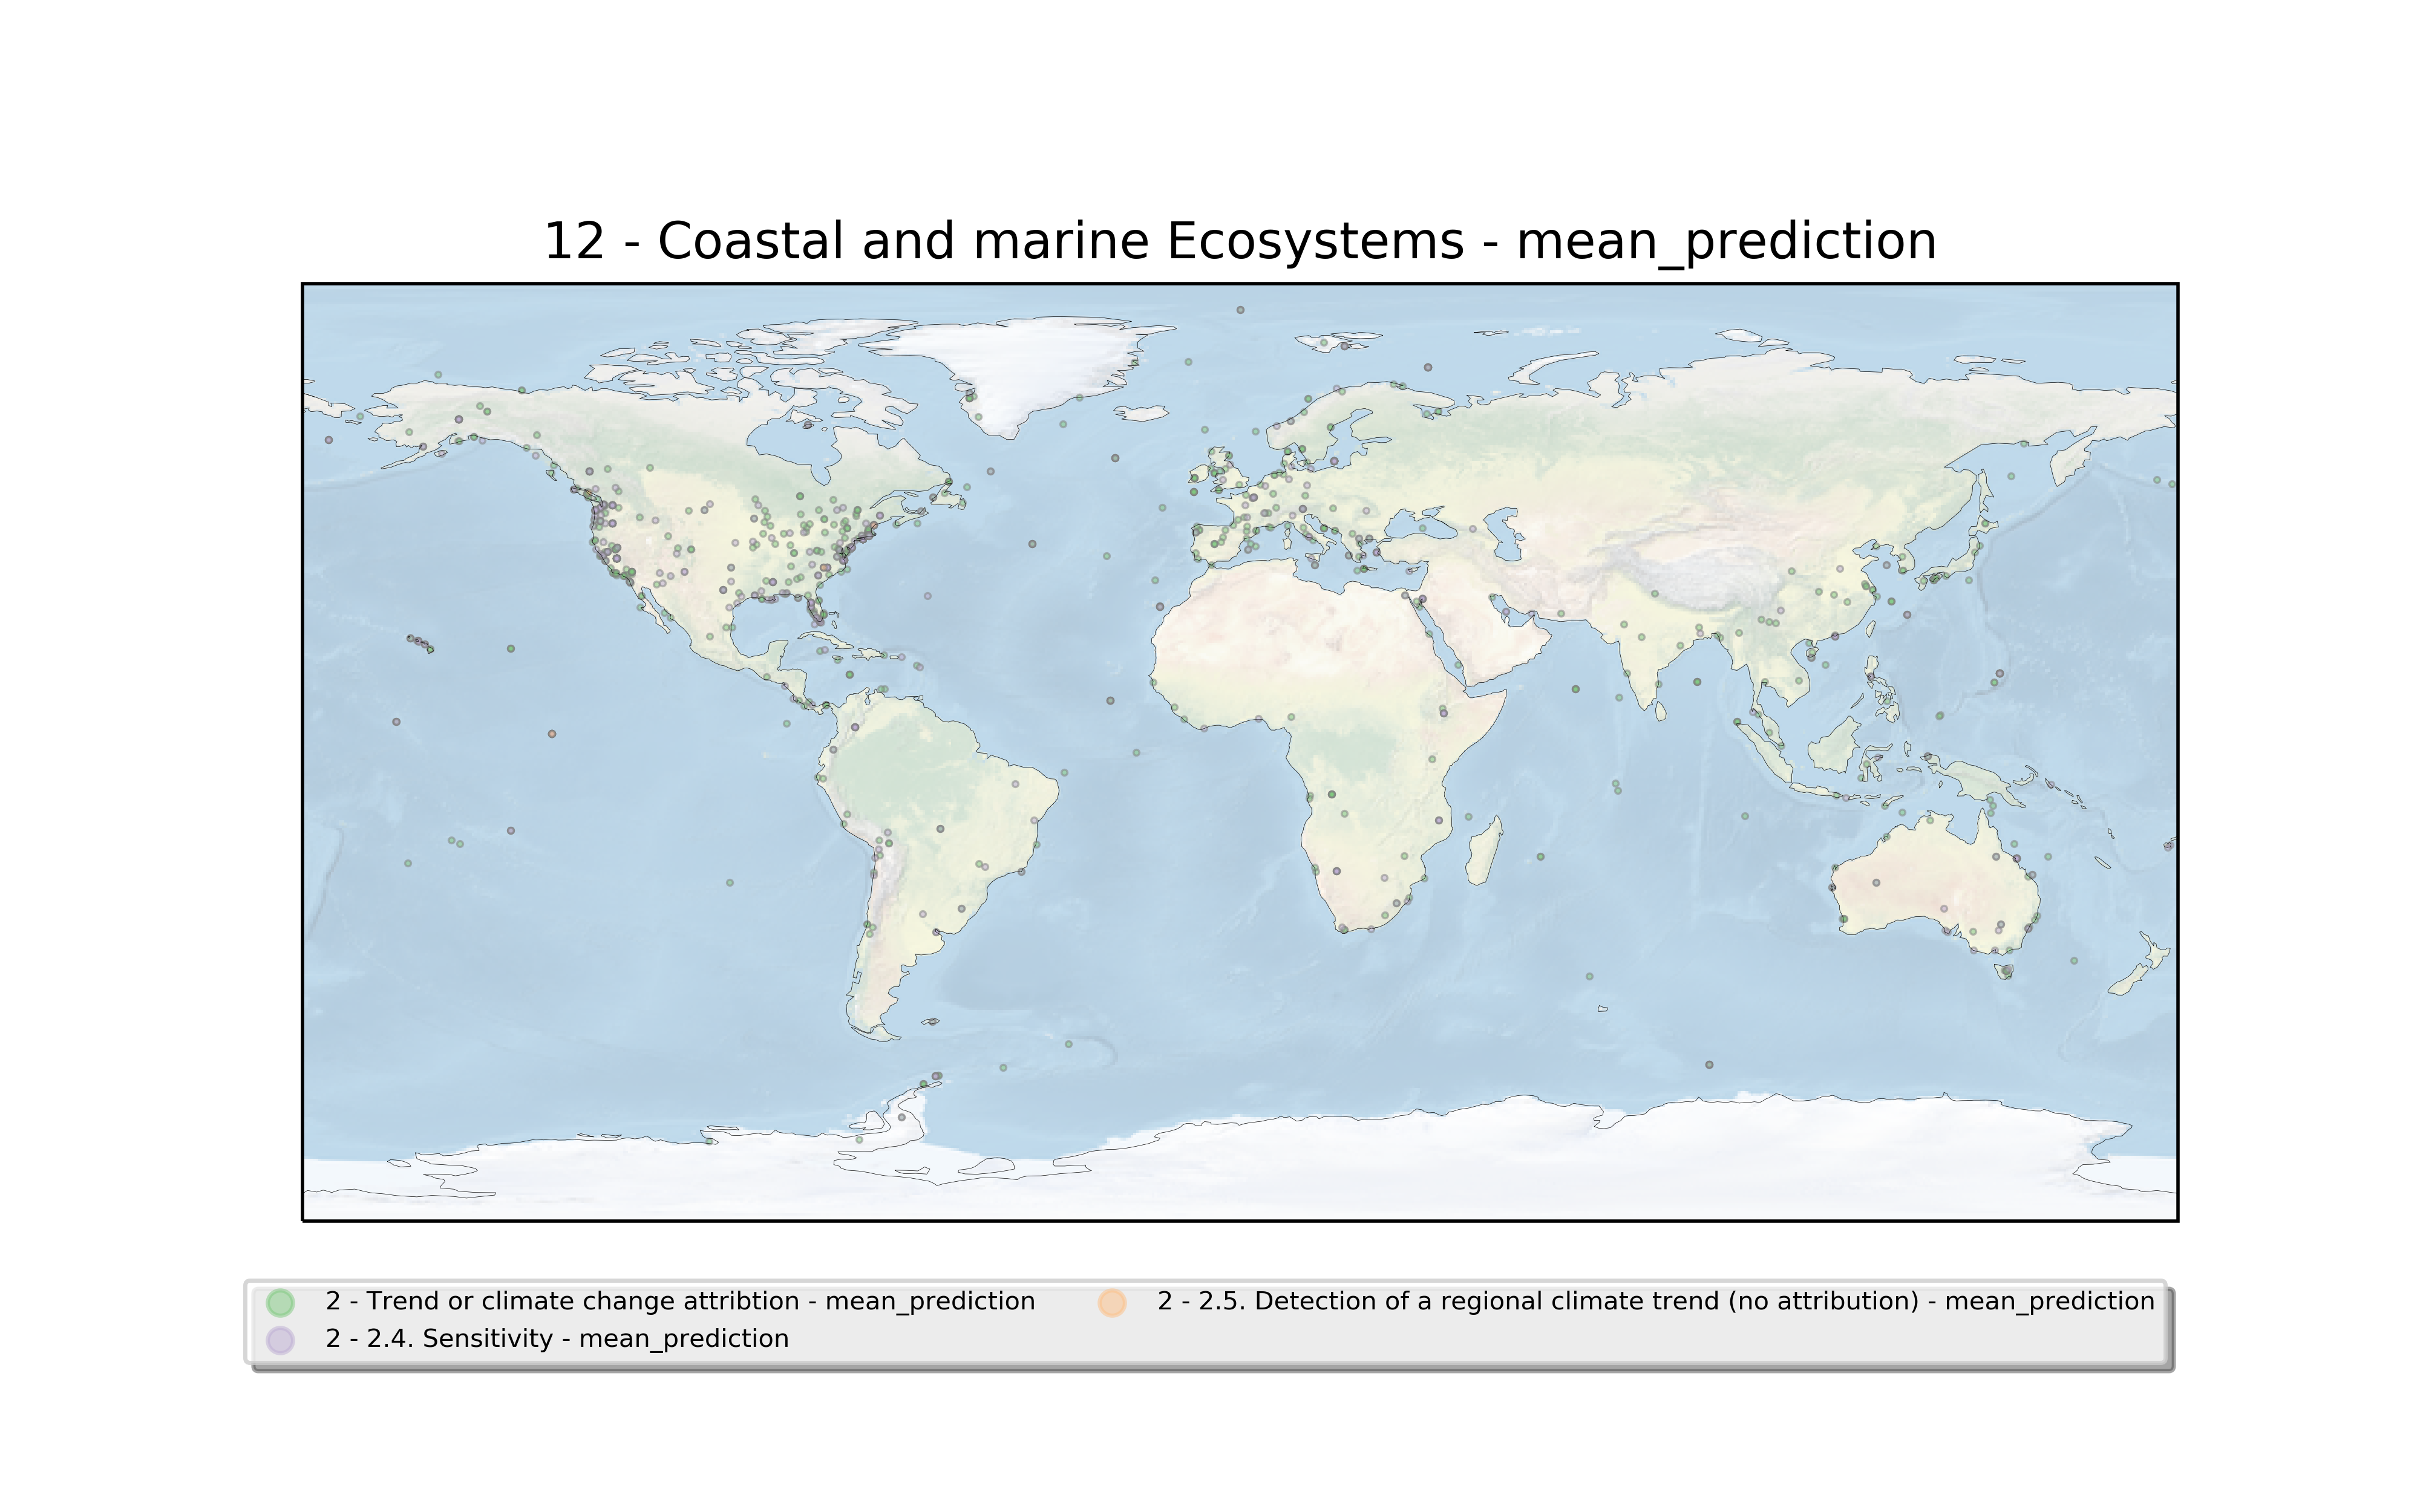
\includegraphics[width=\linewidth]{../plots/maps/predicted_places_Coastal_and_marine_Ecosystems_attribution.png}
	\end{figure}
}
\only<5>{
	\begin{figure}
		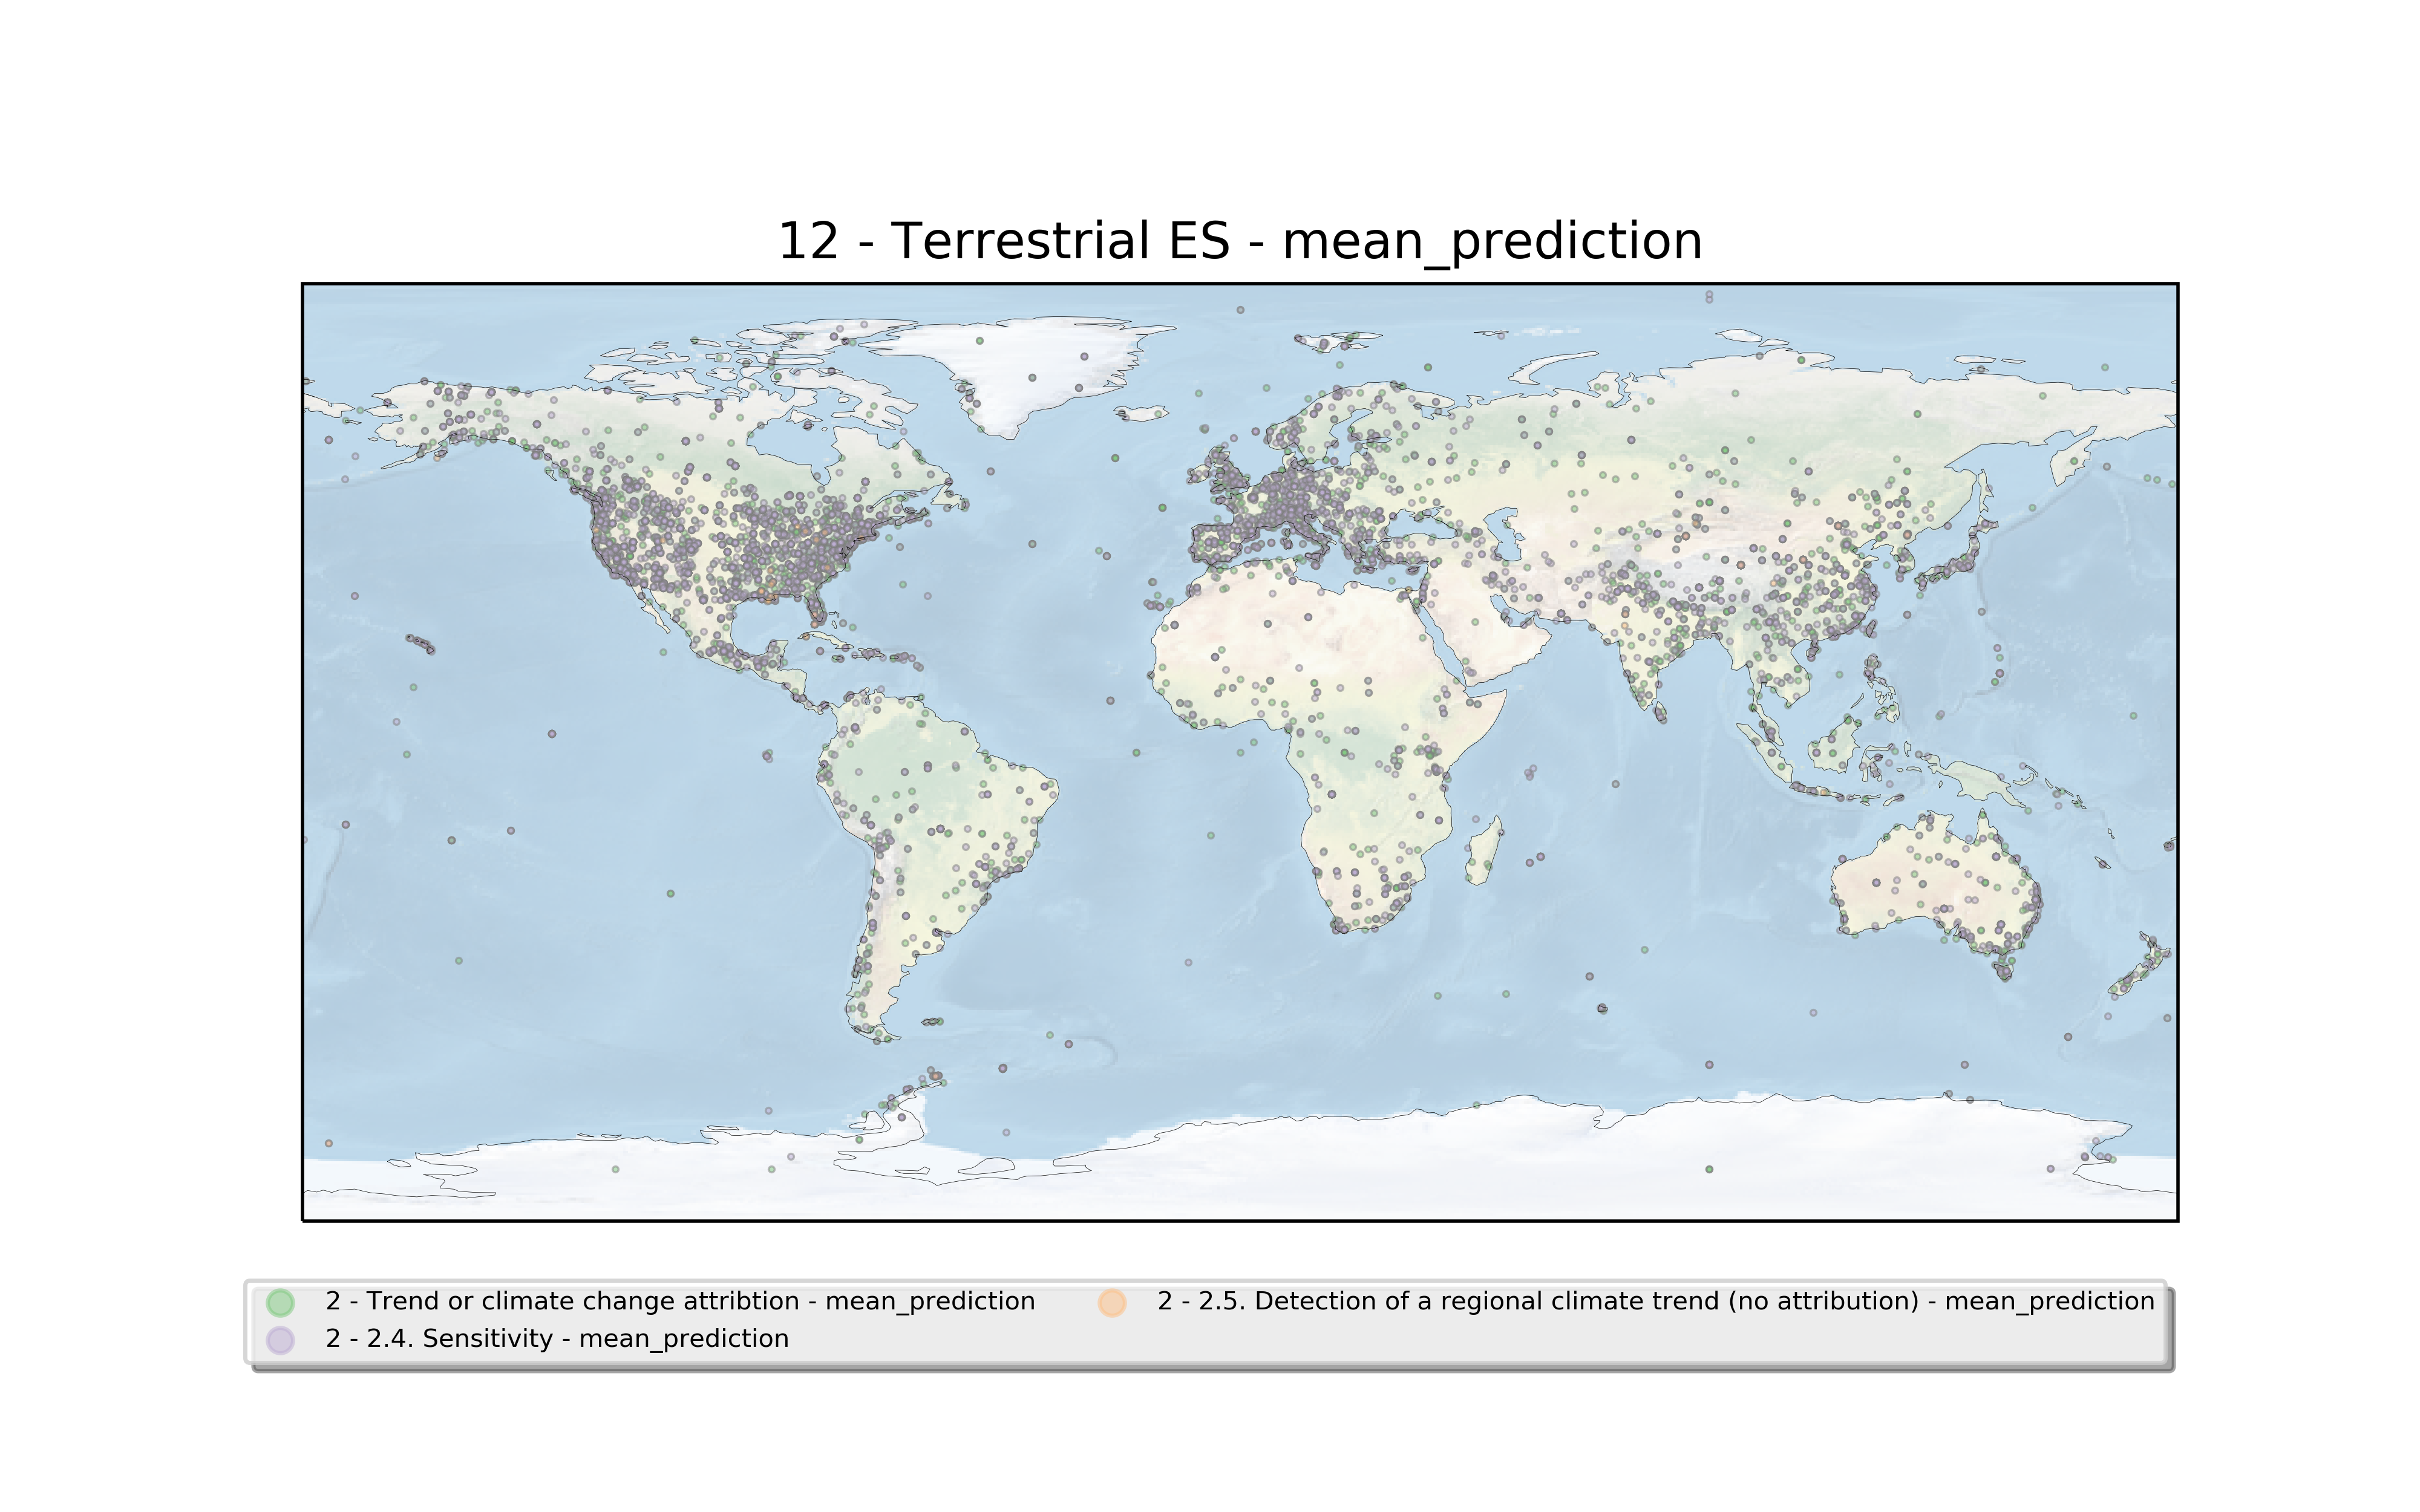
\includegraphics[width=\linewidth]{../plots/maps/predicted_places_Terrestrial_ES_attribution.png}
	\end{figure}
}
\only<6>{
	\begin{figure}
		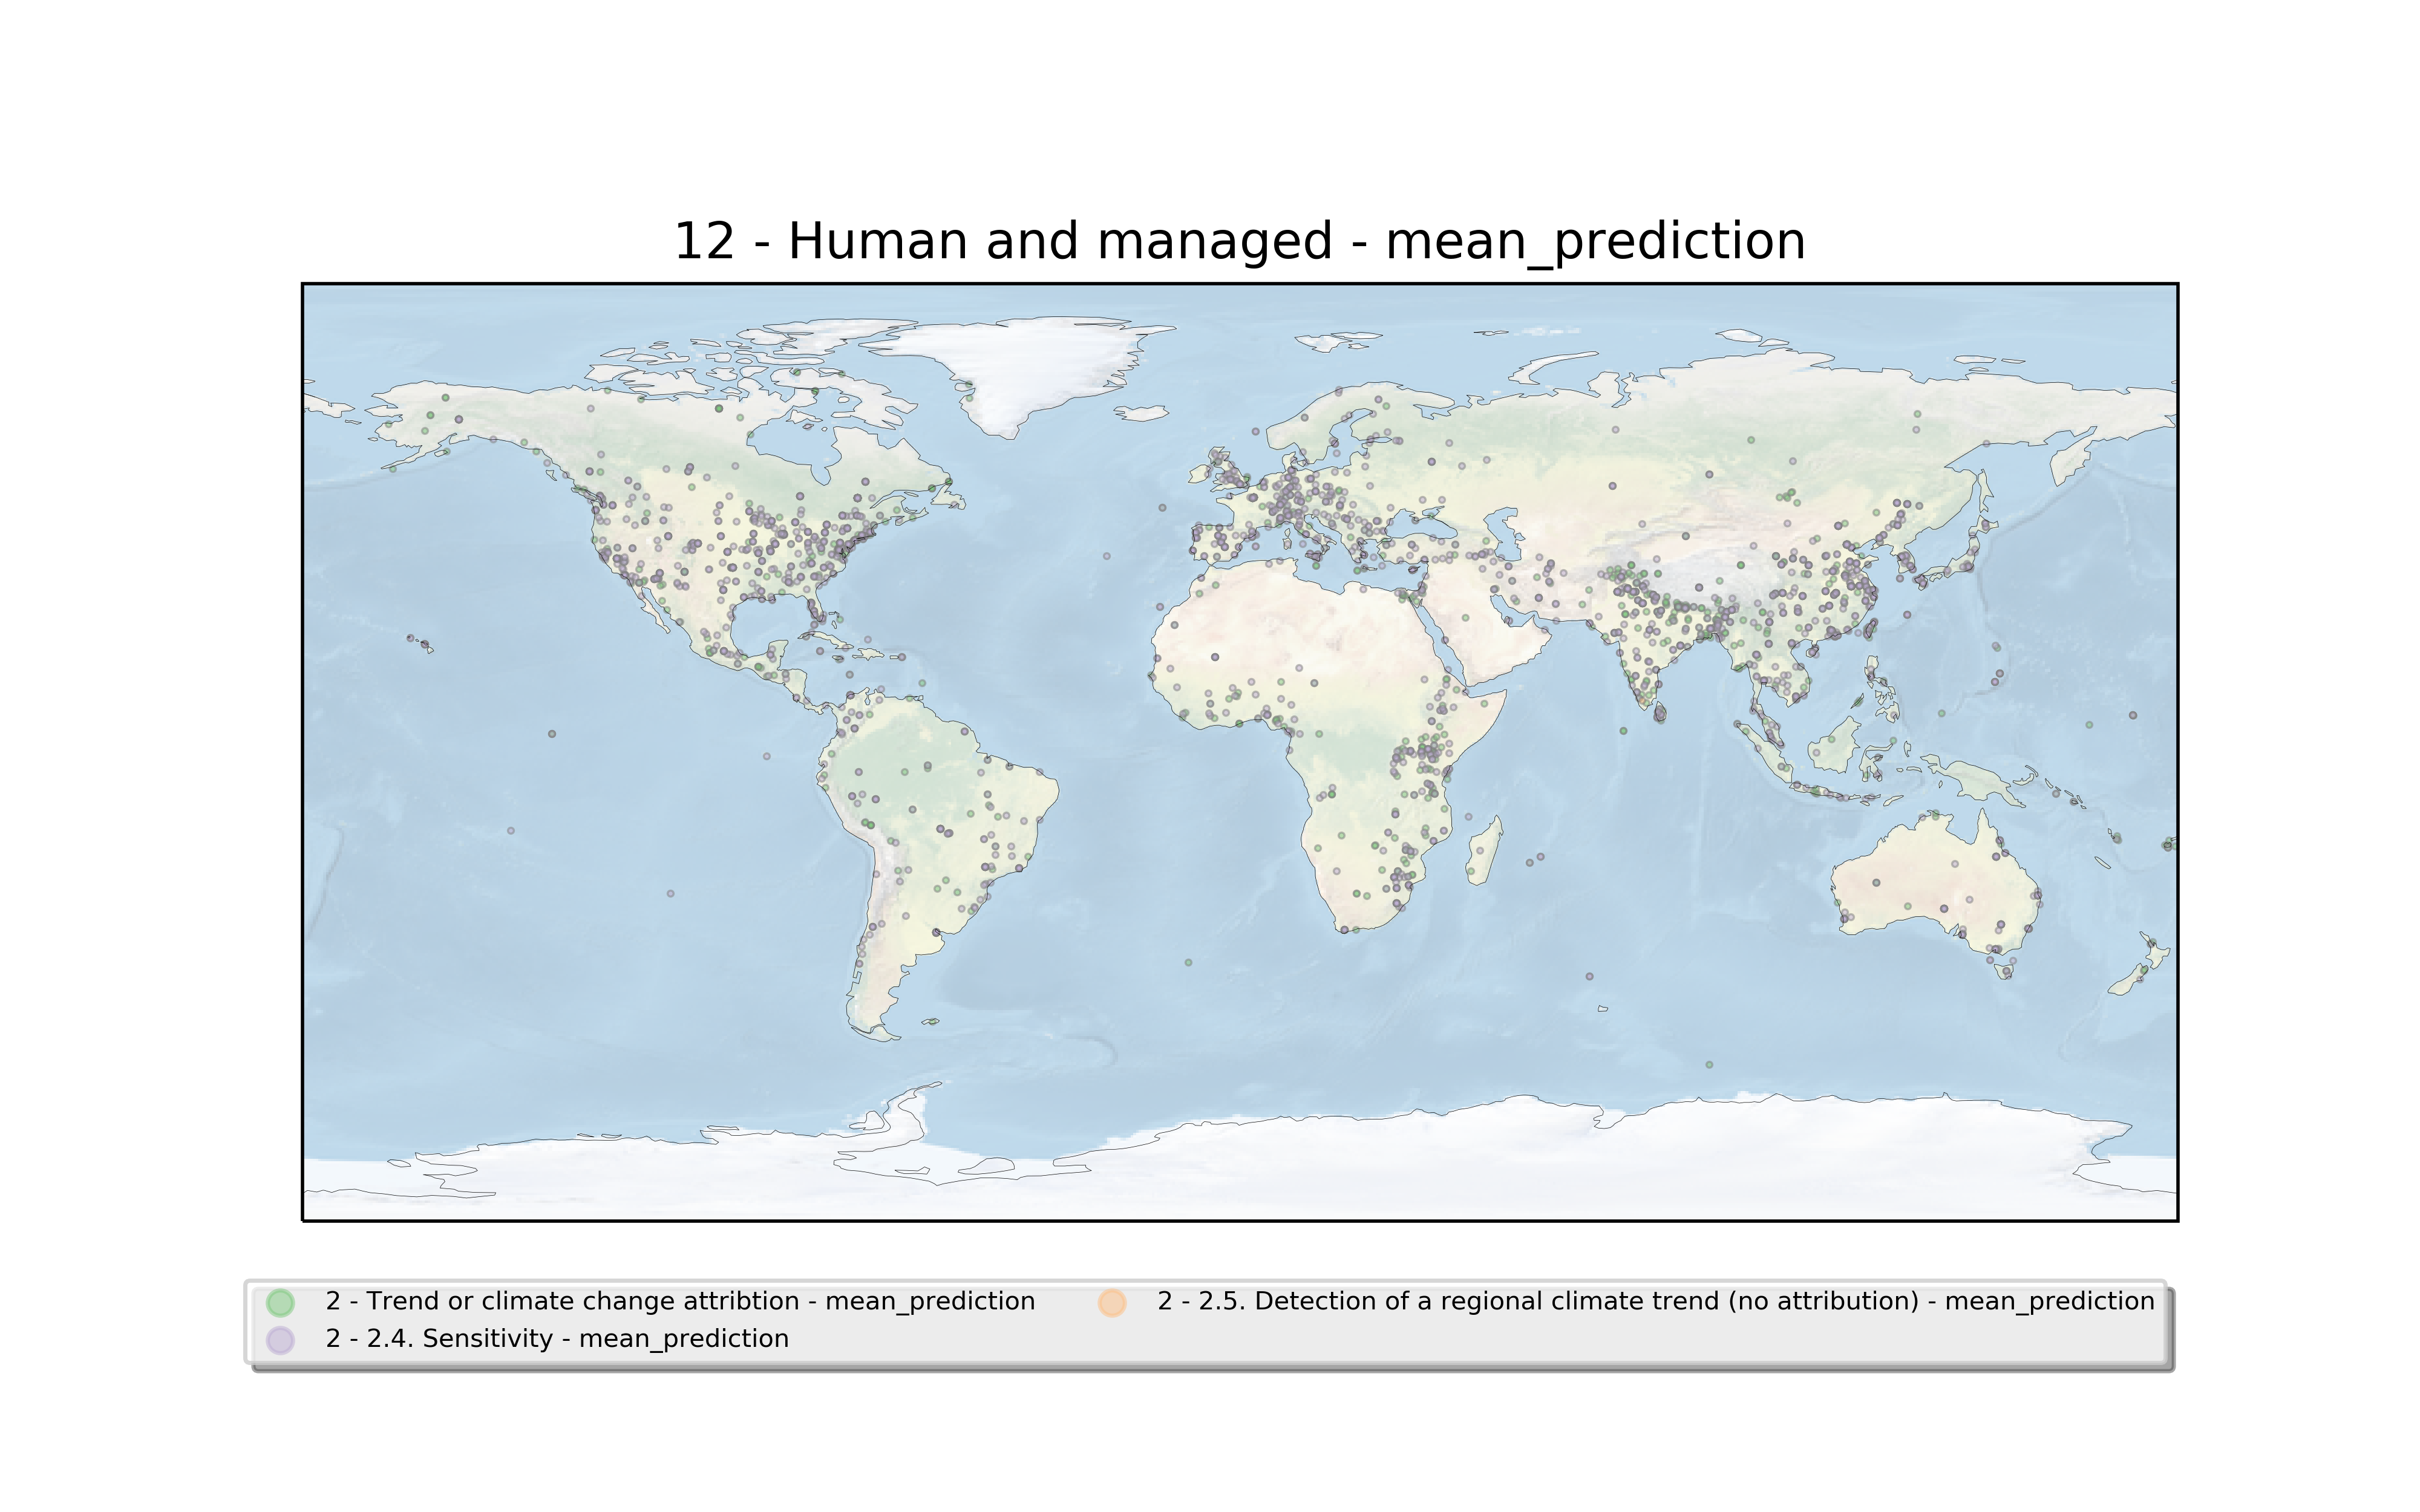
\includegraphics[width=\linewidth]{../plots/maps/predicted_places_Human_and_managed_attribution.png}
	\end{figure}
}
\end{frame}

\begin{frame}{Outlook}
\begin{columns}[t]
	\begin{column}{0.5\linewidth}
		\textbf{So far}
		
		\begin{itemize}
			\item Data collection
			\item Coding scheme
			\item Coding
			\item Learning and predictions
			\item Collation of results
		\end{itemize}
	\end{column}
	\begin{column}{0.5\linewidth}
		\textbf{Still to come}
		\begin{itemize}
			\item Further data checking
			\item Investigating distribution of evidence and comparing with IPCC
			\item Predicting drivers and mapping driver-impact pathways
			\item Write up
			\item Interactive map
		\end{itemize}
	\end{column}
\end{columns}
\end{frame}


\end{document}